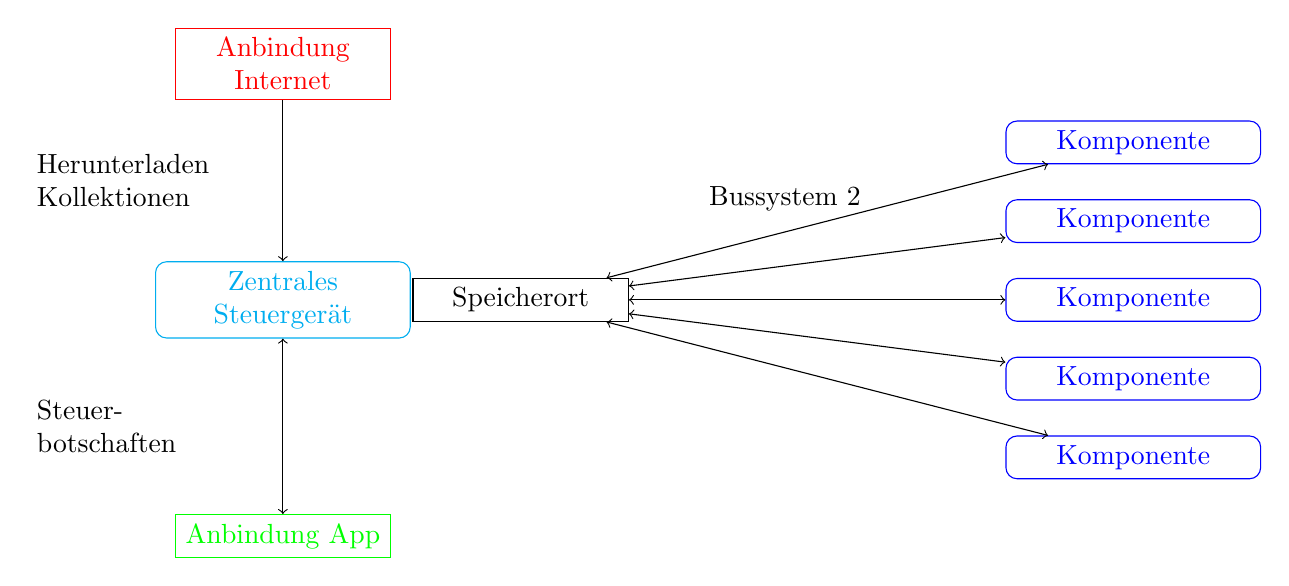
\begin{tikzpicture}[first/.style={draw, text width=3cm, align=center, rounded corners}, second/.style={draw, text width=2.5cm, align=center}]
	\node[first, cyan] (Z) at (0,0) {Zentrales Steuergerät};
	\node[second, red] (C) at (0,3) {Anbindung Internet};
	\node[second, green] (D) at (0,-3) {Anbindung App};
	\node[first, blue] (K1) at (10.8,2) {Komponente};
	\node[first, blue] (K2) at (10.8,1) {Komponente};
	\node[first, blue] (K3) at (10.8,0) {Komponente};
	\node[first, blue] (K4) at (10.8,-1) {Komponente};
	\node[first, blue] (K5) at (10.8,-2) {Komponente};
	\node[second] (S) at (3.02,0) {Speicherort};
	\draw[<-] (Z) -- node[left,text width=3cm] {Herunterladen Kollektionen} (C);
	\draw[<->] (Z) -- node[left,text width=3cm] {Steuer-\\botschaften} (D);
	%\draw[<->] (Z) -- node[above] {Bussystem 1} (S);
	\draw[<->] (S) -- node[above, text width=3cm] {Bussystem 2} (K1);
	\draw[<->] (S) -- (K2);
	\draw[<->] (S) -- (K3);
	\draw[<->] (S) -- (K4);
	\draw[<->] (S) -- (K5);
\end{tikzpicture}